% !TeX program = xelatex
% !TeX encoding = UTF-8
% !TeX TXS-program:compile = txs:///xelatex | txs:///xelatex
\documentclass[aspectratio=169, table, 12pt]{beamer}

% Preamble bersama seluruh slide mata kuliah ini.
% Dipanggil dari slides/sessionXX/sessionXX.tex tepat sesudah baris
% \documentclass[aspectratio=169, table, 12pt]{beamer}
% Paket tambahan yang hanya dibutuhkan satu sesi ditulis di berkas sesi itu.

\usepackage{colortbl}
\usepackage{xcolor}
\usepackage{listings}
\usepackage{tabularx}
\usepackage{booktabs}
\usepackage{tikz}
\usepackage{pgfplots}
\usepackage{fontspec}
\usepackage[english,bahasai]{babel}
\pgfplotsset{compat=1.18}
\usetikzlibrary{arrows.meta, positioning, calc, fit, shapes.geometric,
  shapes.multipart, backgrounds, matrix, chains, trees}

\makeatletter
\def\input@path{{../theme/}}
\makeatother
\graphicspath{{../theme/}{../../figures/}}
% Stub symlink Windows memakai tema cadangan sampai aset institusi tersedia.
\IfFileExists{../theme/beamerthemePradita.sty}{%
  \usetheme{Pradita}
}{%
  \usetheme{Madrid}
  \setmainfont{TeX Gyre Heros}
  \setsansfont{TeX Gyre Heros}
  \setbeamertemplate{navigation symbols}{}
}

\definecolor{praditagreen}{RGB}{37, 113, 71}
\setbeamercolor{structure}{fg=praditagreen}
\setbeamercolor{palette primary}{bg=praditagreen,fg=white}
\setbeamercolor{palette secondary}{bg=praditagreen!80!black,fg=white}
\setbeamercolor{palette tertiary}{bg=praditagreen!60!black,fg=white}
\setbeamerfont{frametitle}{size=\large}
\setbeamertemplate{caption}[numbered]

% Ukuran header mengikuti teks agar judul panjang tidak menabrak logo.
\setbeamercolor{frametitle}{bg=white,fg=black}
\setbeamertemplate{frametitle}{%
  \begin{beamercolorbox}[wd=\paperwidth,sep=0.2cm]{frametitle}
    \begin{minipage}[c]{0.77\paperwidth}
      \raggedright\fontsize{16}{18}\selectfont\bfseries\insertframetitle
      \ifx\insertframesubtitle\empty\else
        \par\small\mdseries\insertframesubtitle
      \fi
    \end{minipage}\hfill
    \begin{minipage}[c]{0.15\paperwidth}
      \IfFileExists{../theme/classFiles/logo_universitas.png}{%
        
\includegraphics[width=\linewidth]{../theme/classFiles/logo_universitas.png}%
      }{}
    \end{minipage}
  \end{beamercolorbox}
}
\setbeamertemplate{footline}{%
  \ifnum\value{framenumber}>1
    \begin{beamercolorbox}[wd=\paperwidth,ht=0.35cm,dp=0.15cm,
      leftskip=0.3cm,rightskip=0.3cm]{palette primary}
      \footnotesize\bfseries\insertframenumber/\inserttotalframenumber
      \hfill IT40513
    \end{beamercolorbox}
  \fi
}
\DeclareRobustCommand{\berkas}[1]{\path{#1}}

% Tema membuat garis tabel berwarna putih. Dikembalikan agar tabel terbaca.
\arrayrulecolor{black}
\setlength{\arrayrulewidth}{0.5pt}

\lstdefinelanguage{yaml}{
  basicstyle=\ttfamily\scriptsize,
  keywordstyle=\color{blue}\bfseries,
  commentstyle=\color{gray}\itshape,
  stringstyle=\color{red},
  showstringspaces=false,
  breaklines=true,
  frame=lines,
  numbers=none,
  backgroundcolor=\color{lightgray!10},
  tabsize=2,
  morecomment=[l]{\#}
}

\lstdefinelanguage{json}{
  basicstyle=\ttfamily\scriptsize,
  stringstyle=\color{red},
  commentstyle=\color{gray},
  breaklines=true,
  showstringspaces=false,
  tabsize=2,
  numbers=none,
  frame=lines,
  backgroundcolor=\color{lightgray!10},
  string=[s]{"}{"}
}

\lstdefinelanguage{bash}{
  keywords={},
  basicstyle=\ttfamily\scriptsize,
  ndkeywords={docker, kubectl, helm, curl, git, terraform},
  ndkeywordstyle=\color{purple}\bfseries,
  sensitive=true,
  commentstyle=\color{gray},
  numbers=none,
  breaklines=true,
  frame=lines,
  backgroundcolor=\color{lightgray!10},
  tabsize=2,
  comment=[l]{\#},
  showstringspaces=false
}

\lstdefinelanguage{http}{
  keywords={GET, POST, PUT, PATCH, DELETE, HEAD, OPTIONS, HTTP},
  basicstyle=\ttfamily\scriptsize,
  keywordstyle=\color{blue}\bfseries,
  sensitive=true,
  numbers=none,
  breaklines=true,
  frame=lines,
  backgroundcolor=\color{lightgray!10},
  tabsize=2,
  showstringspaces=false
}

\subtitle{IT40513 · Enterprise Architecture \& Digital Blueprint}
\author{\textbf{Alfa Yohannis}}


% Sampul membatasi judul di panel putih tema rujukan Pradita.
\setbeamertemplate{title page}{%
  \begin{tikzpicture}[remember picture,overlay]
    \node[anchor=north west,inner sep=0pt,text width=8.8cm]
      at ([xshift=1cm,yshift=-3.15cm]current page.north west) {%
        {\small\insertsubtitle\par}\vspace{0.25cm}
        \resizebox{8.8cm}{!}{\begin{minipage}{12cm}
          \raggedright\color{praditagreen}\bfseries\inserttitle
        \end{minipage}}
      };
    \node[anchor=south west,inner sep=0pt]
      at ([xshift=1cm,yshift=1.65cm]current page.south west)
      {\small\insertdate};
    \node[anchor=west,inner sep=0pt,text=white]
      at ([xshift=0.8cm,yshift=0.75cm]current page.south west)
      {\small\insertauthor};
  \end{tikzpicture}
}


% Batasi kedua dimensi gambar agar diagram bersama tetap berada pada slide.
\newsavebox{\eafigbox}
\newcommand{\eadiagram}[1]{%
  \sbox{\eafigbox}{\resizebox{0.94\textwidth}{!}{\input{#1}}}%
  \ifdim\dimexpr\ht\eafigbox+\dp\eafigbox\relax>0.64\textheight
    \resizebox{!}{0.64\textheight}{\usebox{\eafigbox}}%
  \else
    \usebox{\eafigbox}%
  \fi
}


\newcolumntype{Y}{>{\raggedright\arraybackslash}X}
\newcolumntype{L}[1]{>{\raggedright\arraybackslash}p{#1}}

% Font tema slide lebih lebar daripada font modul, sehingga kotak diagram jalur kritis
% bertumpuk. Lebar kotak dan jarak tegaknya dilonggarkan khusus di slide ini.
\makeatletter
\newcommand{\longgarkandiagram}[2]{%
  \tikzset{text width/.code={\def\tikz@text@width{#1}},
           every picture/.append style={y=#2}}}
\makeatother

\title{\Huge Transisi, Peta Jalan,\\ \vspace{10pt} dan Perencanaan Migrasi}
\date{Pertemuan 12}

\begin{document}

\frame{\titlepage}

\begin{frame}
  \frametitle{Isi Pertemuan}
  \vspace{14pt}
  \begin{columns}[t]
    \column{0.5\textwidth}
    {\small\tableofcontents[sections={1-3}]}

    \column{0.5\textwidth}
    {\small\tableofcontents[sections={4-6}]}
  \end{columns}
\end{frame}

\begin{frame}{\hfill}
  \centering
  \Huge{\textbf{Bila program berhenti\\di tengah jalan, apa yang\\tersisa bagi organisasi?}}
\end{frame}

\section{Tujuan dan Konteks}

\begin{frame}{\hfill}
  \centering
  \Huge{\textbf{Tujuan dan Konteks}}
\end{frame}

\begin{frame}{{\Large Tujuan Pembelajaran}}
  \vspace{10pt}
  \begin{itemize}
    \item Merancang dua sampai tiga arsitektur transisi yang masing-masing memberi nilai bisnis.
    \item Menyusun peta jalan 2026 sampai 2030 berdasarkan dependensi, nilai, risiko, dan kapasitas
          organisasi.
    \item Menyusun rencana migrasi tingkat tinggi beserta asumsi dan titik keputusannya.
  \end{itemize}
\end{frame}

\begin{frame}{{\Large Masalah: Program Raksasa Menumpuk Risiko}}
  \small
  \vspace{4pt}
  \begin{itemize}
    \item Godaan setelah Bab 11: identitas pasien, kontrol akses, konsolidasi Sistem Informasi
          Manajemen Rumah Sakit (SIMRS), dan lainnya dikerjakan sekaligus.
    \item Bila berhenti di tengah, organisasi sudah membayar mahal tanpa hasil yang dapat dipakai.
    \item Flyvbjerg dan Budzier meneliti 1.471 proyek teknologi informasi (TI): pembengkakan biaya
          rata-rata 27 persen.
    \item Satu dari enam proyek membengkak rata-rata 200 persen, dengan keterlambatan hampir 70 persen.
    \item Fase E dan fase F dalam ADM (\textit{Architecture Development Method}) memecahnya menjadi
          langkah yang selesai dan bermanfaat.
  \end{itemize}
\end{frame}

\section{Arsitektur Transisi}

\begin{frame}{\hfill}
  \centering
  \Huge{\textbf{Arsitektur Transisi}}
\end{frame}

\begin{frame}{{\Large Apa Itu Arsitektur Transisi}}
  \small
  \vspace{6pt}
  \begin{itemize}
    \item Gambaran formal arsitektur pada satu titik waktu penting di antara kondisi saat ini dan
          kondisi target.
    \item Domainnya sama dengan target: bisnis, data, aplikasi, dan teknologi.
    \item ArchiMate menyebutnya \textit{plateau}: keadaan yang relatif stabil selama kurun waktu
          tertentu.
    \item Setiap pijakan dijalankan sehari-hari, bukan sekadar tanggal di jadwal proyek.
  \end{itemize}
  \vspace{6pt}
  Analogi: merenovasi rumah yang tetap dihuni. Bila uang habis setelah tahap kedua, kamar mandi baru
  tetap berfungsi.
\end{frame}

\begin{frame}{{\Large Diagram Konsep Bab 12}}
  \centering
  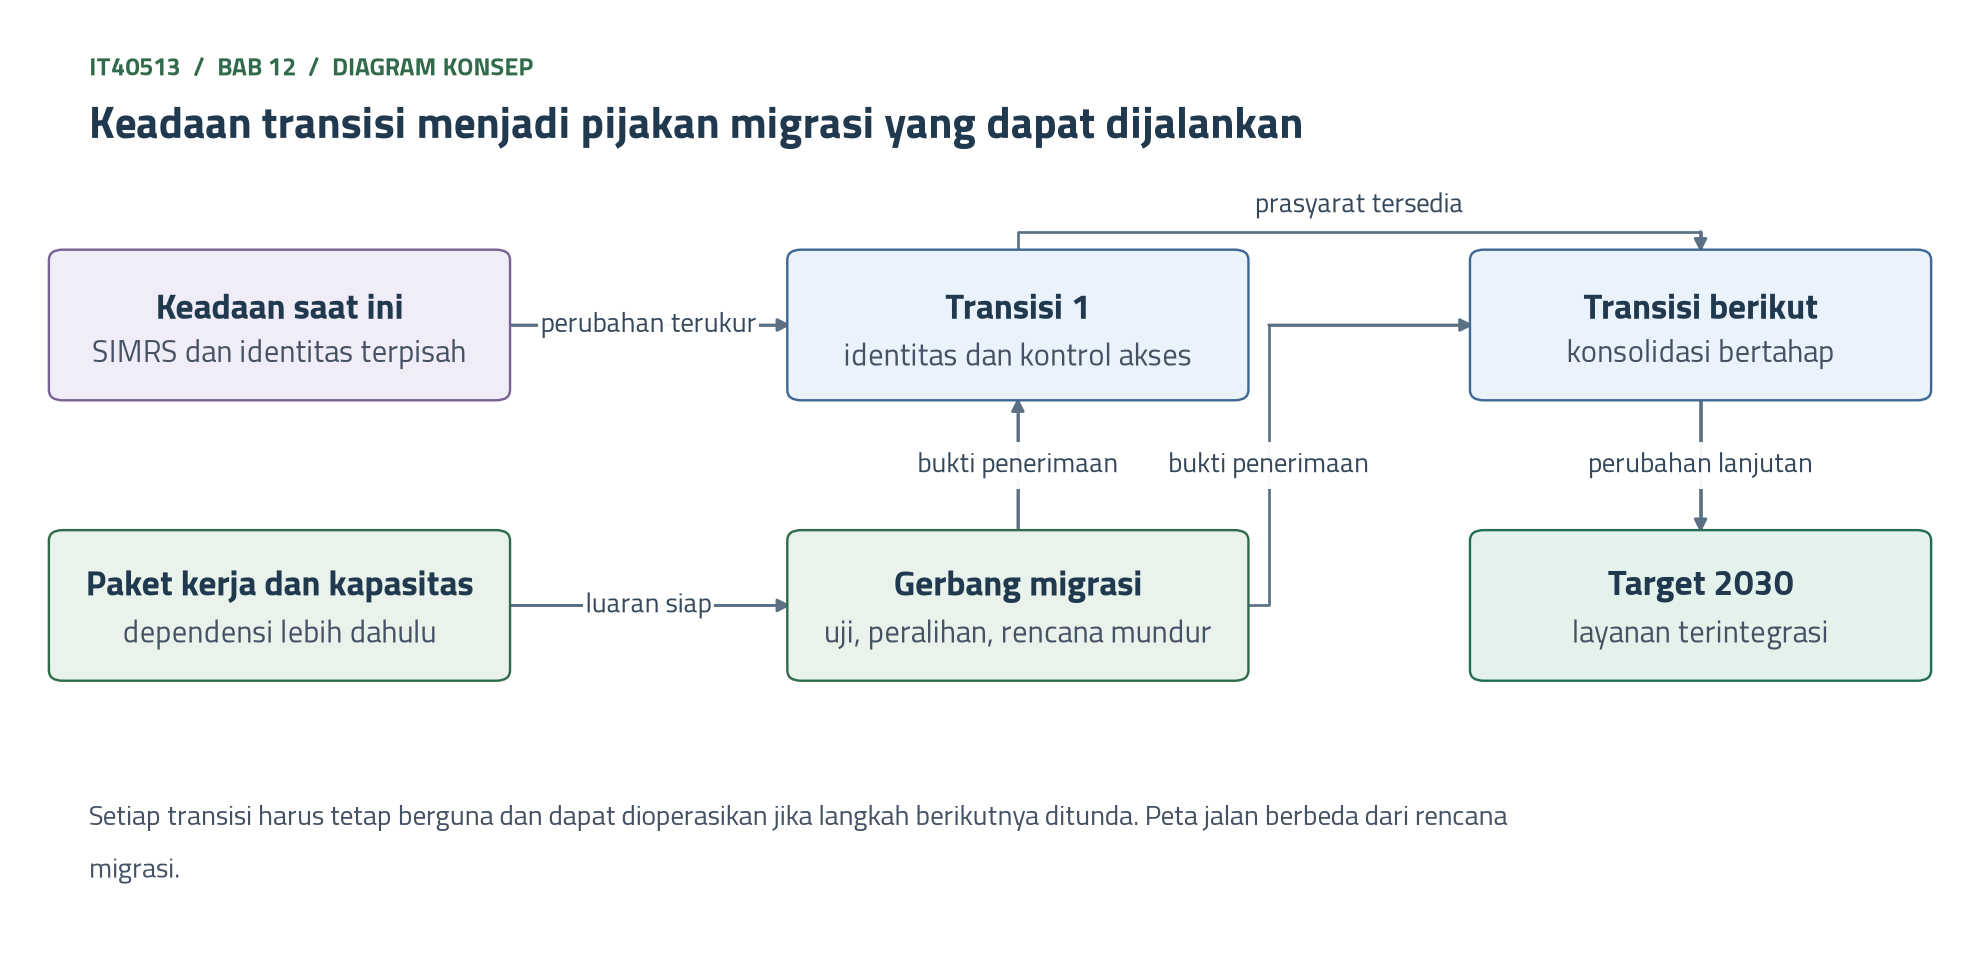
\includegraphics[width=0.96\textwidth,height=0.77\textheight,keepaspectratio]{../../figures/ch12-diagram-konsep.png}
  \label{fig:session12-ilustrasi-bab}
\end{frame}

\begin{frame}{{\Large Empat Syarat Transisi yang Bernilai}}
  \scriptsize
  \begin{tabularx}{\textwidth}{L{2.6cm}YY}
    \hline
    \textbf{Syarat} & \textbf{Pertanyaan uji} & \textbf{Contoh yang gagal} \\
    \hline
    Memberi manfaat yang terlihat & Siapa yang merasakan perubahannya, dan
      dengan ukuran apa? & \textit{Cloud} sudah siap, tetapi belum ada
      aplikasi yang pindah \\
    \hline
    Stabil bila langkah berikutnya ditunda & Bila langkah berikutnya mundur
      dua tahun, apakah keadaan ini tetap berjalan dengan biaya wajar? & Data
      pasien baru separuh dipindahkan, sehingga dua sumber data berjalan
      bersamaan \\
    \hline
    Searah dengan target & Adakah bagian yang harus dibongkar lagi untuk
      mencapai target? & SIMRS lama ditingkatkan besar-besaran, padahal akan
      diganti dua tahun kemudian \\
    \hline
    Dapat dinyatakan tercapai & Adakah ukuran yang jelas untuk menyatakan
      transisi ini tercapai? & Transisi bernama ``Digitalisasi Tahap 1''
      tanpa daftar kemampuan dan ukuran \\
    \hline
  \end{tabularx}

  \vspace{6pt}
  \small Syarat kedua paling sering dilanggar.
\end{frame}

\begin{frame}{{\Large Uji Penundaan dan Jumlah Transisi}}
  \small
  \vspace{4pt}
  \begin{itemize}
    \item Uji penundaan: andaikan langkah berikutnya ditunda dua tahun, lalu hitung apa yang tersisa.
    \item Pekerjaan sementara dianggarkan secara sadar, misalnya antarmuka sistem lama dan baru.
    \item Batas transisi jatuh sesudah paket yang tidak boleh berhenti di tengah.
    \item Horizon empat sampai lima tahun cukup dua sampai tiga transisi, berjarak 9 sampai 24 bulan.
    \item Misalkan stabilisasi tiga bulan. Lima transisi dalam 54 bulan menghabiskan hampir 28 persen
          waktu, tiga transisi sekitar 17 persen.
  \end{itemize}
\end{frame}

\begin{frame}{{\Large Transisi yang Lolos dan yang Gagal}}
  \small
  \vspace{6pt}
  \begin{itemize}
    \item Misalkan kabupaten menyatukan 40 aplikasi perizinan ke satu portal dalam empat tahun.
    \item Transisi pertama: satu akun warga dan satu nomor permohonan untuk 12 izin tersering. Bila
          tahap berikutnya ditunda, satu pintu itu tetap ada.
    \item Misalkan perusahaan distribusi dengan 25 gudang memindahkan basis data ke \textit{cloud} tanpa
          mengubah aplikasi.
    \item Sewa naik, misalnya Rp1,2 miliar per tahun, tetapi tidak ada proses gudang yang berubah.
    \item Bila penggantian aplikasi ditunda dua tahun, Rp2,4 miliar terbayar tanpa manfaat.
  \end{itemize}
\end{frame}

\begin{frame}{{\Large Tiga Transisi Medikara}}
  \centering
  \begin{figure}
    \resizebox{0.94\textwidth}{!}{\begin{tikzpicture}[
  font=\scriptsize,
  tahap/.style={draw, rounded corners, minimum height=1.25cm, text width=1.62cm,
                align=center, font=\scriptsize\bfseries},
  baris/.style={text width=1.12cm, align=right, font=\tiny\bfseries},
  isi/.style={text width=1.72cm, align=center, font=\tiny},
  panah/.style={-{Stealth[length=2mm]}, thick}
]
  \node[tahap, fill=gray!35] (awal) at (0,0)
    {Kondisi awal\\[2pt]{\tiny\mdseries Juli 2026}};
  \node[tahap, fill=blue!8] (t1) at (2.2,0)
    {T1: Pasien dan akses\\[2pt]{\tiny\mdseries Maret 2028}};
  \node[tahap, fill=blue!8] (t2) at (4.4,0)
    {T2: Rekam medis tahap awal\\[2pt]{\tiny\mdseries Maret 2029}};
  \node[tahap, fill=blue!8] (t3) at (6.6,0)
    {T3: Ekosistem mitra\\[2pt]{\tiny\mdseries Desember 2029}};
  \node[tahap, fill=green!10] (target) at (8.8,0)
    {Target: satu rekam medis\\[2pt]{\tiny\mdseries September 2030}};

  \draw[panah] (awal) -- (t1);
  \draw[panah] (t1) -- (t2);
  \draw[panah] (t2) -- (t3);
  \draw[panah] (t3) -- (target);

  \node[baris] at (-1.55,-1.15) {Paket yang selesai};
  \node[isi] at (0,-1.15) {lima SIMRS, integrasi \textit{point-to-point}};
  \node[isi] at (2.2,-1.15) {P1, P2, P3, P4};
  \node[isi] at (4.4,-1.15) {P6, P7, dan P5 di Depok};
  \node[isi] at (6.6,-1.15) {P8, dan P5 di tiga rumah sakit};
  \node[isi] at (8.8,-1.15) {P5 di lima rumah sakit};

  \draw[gray!60] (-2.15,-1.68) -- (9.7,-1.68);

  \node[baris] at (-1.55,-2.25) {Tersisa bila berhenti di sini};
  \node[isi] at (0,-2.25) {temuan audit terbuka, data pasien ganda};
  \node[isi] at (2.2,-2.25) {satu nomor pasien, akses terkendali};
  \node[isi] at (4.4,-2.25) {antrean daring, laporan tanpa \textit{spreadsheet}};
  \node[isi] at (6.6,-2.25) {mitra terhubung lewat API};
  \node[isi] at (8.8,-2.25) {satu rekam medis untuk tiap pasien};
\end{tikzpicture}
}
    \caption{Tiga arsitektur transisi Medikara menuju target 2030. Kode P1 sampai P8 adalah paket
             kerja}
  \end{figure}
\end{frame}

\begin{frame}{{\Large Transisi Pertama: Identitas dan Akses}}
  \begin{block}{Kasus Medikara Health}
    \small
    \begin{itemize}
      \item Pemicu mendesak: insiden 2025 dan temuan audit belum tertutup. Kewajiban Undang-Undang
            Pelindungan Data Pribadi (UU PDP) berlaku penuh sejak Oktober 2024.
      \item Paket lain bergantung: konsolidasi SIMRS butuh satu identitas pasien.
      \item Lolos uji penundaan: satu nomor pasien untuk 5 rumah sakit dan 18 klinik, akses 4.800
            karyawan dari satu tempat, dan satu \textit{hub} integrasi.
      \item Misalkan lima adaptor masing-masing Rp150 juta per tahun. Bila T2 tertunda dua tahun,
            biayanya Rp1,5 miliar.
    \end{itemize}
  \end{block}
\end{frame}

\section{Mengurutkan Paket Kerja}

\begin{frame}{\hfill}
  \centering
  \Huge{\textbf{Mengurutkan Paket Kerja}}
\end{frame}

\begin{frame}{{\Large Empat Kriteria Pengurutan}}
  \scriptsize
  \begin{tabularx}{\textwidth}{L{1.6cm}YL{2.8cm}L{3.0cm}}
    \hline
    \textbf{Kriteria} & \textbf{Pertanyaan} & \textbf{Sifat} & \textbf{Sumber data} \\
    \hline
    Dependensi & Paket apa yang harus selesai sebelum paket ini dimulai? &
      Syarat mutlak & Matriks dependensi Bab 11 \\
    \hline
    Nilai & Seberapa besar manfaat yang dirasakan pasien atau manajemen? &
      Skor 1 sampai 5 & Rantai motivasi Bab 3, \textit{heatmap} Bab 5 \\
    \hline
    Risiko & Seberapa besar risiko organisasi yang turun bila paket selesai?
      Seberapa sulit paket itu dikerjakan? & Skor 1 sampai 5, ditambah
      catatan risiko pelaksanaan & Temuan audit, daftar risiko IT40813 \\
    \hline
    Kapasitas & Berapa paket besar yang sanggup dikerjakan dalam setahun? &
      Batas per tahun & Jumlah staf TI, vendor, kesiapan unit bisnis \\
    \hline
  \end{tabularx}

  \vspace{6pt}
  \small Keempatnya tidak setara. Dependensi tidak dapat ditawar, skor memilih di antara paket yang
  sama-sama siap, dan kapasitas membatasi jumlahnya.
\end{frame}

\begin{frame}{{\Large Kriteria Diterapkan Berurutan}}
  \small Analogi: juru masak hajatan. Nasi ditanak sebelum tumpeng dibentuk (dependensi), hidangan yang
  ditunggu tamu lebih dahulu (nilai), masakan yang mudah gagal dikerjakan pagi hari (risiko), dan
  dapur hanya punya dua kompor besar (kapasitas).

  \centering
  \begin{figure}
    \resizebox{0.94\textwidth}{!}{\begin{tikzpicture}[
  font=\scriptsize,
  kotak/.style={draw, rounded corners, minimum height=1.0cm, text width=1.45cm,
                align=center, font=\scriptsize\bfseries},
  tanya/.style={text width=1.6cm, align=center, font=\tiny},
  panah/.style={-{Stealth[length=2mm]}, thick}
]
  \node[kotak, fill=praditagreen!15] (daftar) at (0,0)
    {Paket kerja\\{\tiny\mdseries dari Bab 11}};
  \node[kotak, fill=blue!8] (dep) at (2.05,0)
    {Dependensi\\{\tiny\mdseries syarat mutlak}};
  \node[kotak, fill=blue!8] (nilai) at (4.1,0)
    {Nilai dan risiko\\{\tiny\mdseries skor}};
  \node[kotak, fill=orange!12] (kap) at (6.15,0)
    {Kapasitas\\{\tiny\mdseries batas per tahun}};
  \node[kotak, fill=blue!8] (angg) at (8.2,0)
    {Anggaran\\{\tiny\mdseries titik keputusan}};
  \node[kotak, fill=green!10] (peta) at (10.25,0)
    {Peta jalan\\{\tiny\mdseries 2026 sampai 2030}};

  \draw[panah] (daftar) -- (dep);
  \draw[panah] (dep) -- (nilai);
  \draw[panah] (nilai) -- (kap);
  \draw[panah] (kap) -- (angg);
  \draw[panah] (angg) -- (peta);

  \node[tanya, anchor=north] at (0,-0.7) {6 sampai 10 paket beserta matriks dependensi};
  \node[tanya, anchor=north] at (2.05,-0.7) {Apa yang harus selesai lebih dahulu?};
  \node[tanya, anchor=north] at (4.1,-0.7)
    {Mana yang paling bermanfaat dan paling menurunkan risiko?};
  \node[tanya, anchor=north] at (6.15,-0.7)
    {Berapa proyek besar yang sanggup berjalan dalam setahun?};
  \node[tanya, anchor=north] at (8.2,-0.7) {Kapan dana tahun berikutnya diputuskan?};
  \node[tanya, anchor=north] at (10.25,-0.7) {Urutan, transisi, dan titik keputusan};
\end{tikzpicture}
}
    \caption{Dependensi menyaring, skor memilih, kapasitas membatasi, dan siklus anggaran menetapkan
             titik keputusan}
  \end{figure}
\end{frame}

\begin{frame}{{\Large Delapan Paket Kerja Medikara}}
  \scriptsize
  \begin{tabularx}{\textwidth}{lYlrlrrr}
    \hline
    \textbf{Kode} & \textbf{Paket kerja} & \textbf{Ukuran} & \textbf{Bulan} &
      \textbf{Pendahulu} & \textbf{Nilai} & \textbf{Risiko} & \textbf{Skor} \\
    \hline
    P1 & Kontrol akses terpusat & besar & 9 & tidak ada & 3 & 5 & 8 \\
    \hline
    P2 & \textit{Hub} integrasi BPJS dan SATUSEHAT & sedang & 6 & tidak ada & 3 & 3 & 6 \\
    \hline
    P3 & Identitas pasien tunggal (MPI) & besar & 12 & P1, P2 & 5 & 4 & 9 \\
    \hline
    P4 & \textit{Landing zone} \textit{cloud} & sedang & 6 & P1 & 1 & 2 & 3 \\
    \hline
    P5 & Konsolidasi SIMRS & besar & 30 & P3, P4 & 5 & 3 & 8 \\
    \hline
    P6 & Laporan manajemen terpadu & sedang & 12 & P3, P4 & 4 & 2 & 6 \\
    \hline
    P7 & Antrean dan janji temu lintas fasilitas & sedang & 9 & P2, P3 & 4 & 1 & 5 \\
    \hline
    P8 & Portal dan API mitra & besar & 12 & P2, P3 & 4 & 1 & 5 \\
    \hline
  \end{tabularx}

  \vspace{6pt}
  \small Skor prioritas adalah jumlah skor nilai dan skor pengurangan risiko.
\end{frame}

\begin{frame}{{\Large Skor, Fondasi, dan Hasil Cepat}}
  \small
  \vspace{4pt}
  \begin{itemize}
    \item P3 punya skor tertinggi, yaitu 9, tetapi menunggu P1 dan P2.
    \item P4 punya skor terendah, yaitu 3, tetapi P5 dan P6 menunggunya. Skor tidak pernah boleh
          mengalahkan dependensi.
    \item Fondasi: nilainya kecil bila berdiri sendiri, tetapi menjadi syarat banyak paket. Contohnya
          P2 dan P4.
    \item Hasil cepat (\textit{quick win}): manfaatnya cepat terlihat dan dependensinya sedikit.
          Contohnya P7.
    \item Setiap transisi memuat paling sedikit satu hasil yang terlihat, dan hasil cepat harus searah
          dengan target.
  \end{itemize}
\end{frame}

\begin{frame}{{\Large Kapasitas dan Siklus Anggaran}}
  \small
  \vspace{4pt}
  \begin{itemize}
    \item Tim TI hanya sanggup dua proyek besar per tahun, dihitung pada setiap tahun yang dilaluinya.
    \item Bila semua dimulai sedini mungkin, 2028 memuat tiga: P3, P5, dan P8. P8 bergeser ke Januari
          2029.
    \item Target tetap September 2030. Bila P5 yang digeser, target ikut mundur.
    \item Misalkan tahun anggaran Januari sampai Desember. Pendanaan paket yang mulai April 2028 masuk
          usulan Oktober 2027.
    \item Karena itu P4 dijadwalkan selesai September 2027, sebulan sebelum keputusan pendanaan P5.
  \end{itemize}
\end{frame}

\begin{frame}{{\Large Pendalaman: Jalur Kritis}}
  \centering
  \begin{figure}
    {\longgarkandiagram{2.45cm}{1.15cm}%
    \resizebox{!}{0.56\textheight}{\begin{tikzpicture}[
  font=\scriptsize,
  paket/.style={draw, rounded corners, minimum height=0.95cm, text width=2.45cm,
                align=center, font=\scriptsize\bfseries},
  panah/.style={-{Stealth[length=2mm]}, thick},
  kritis/.style={-{Stealth[length=2mm]}, very thick, orange!80!black}
]
  \node[paket, fill=orange!12] (p1) at (0,1.2)
    {P1 Kontrol akses\\{\tiny\mdseries 9 bulan, 0 sampai 9\\longgar 0}};
  \node[paket, fill=blue!8] (p2) at (0,-1.6)
    {P2 Hub integrasi\\{\tiny\mdseries 6 bulan, 0 sampai 6\\longgar 3}};
  \node[paket, fill=orange!12] (p3) at (3.15,0)
    {P3 Identitas pasien\\{\tiny\mdseries 12 bulan, 9 sampai 21\\longgar 0}};
  \node[paket, fill=blue!8] (p4) at (3.15,2.0)
    {P4 \textit{Landing zone}\\{\tiny\mdseries 6 bulan, 9 sampai 15\\longgar 6}};
  \node[paket, fill=orange!12] (p5) at (6.3,2.4)
    {P5 SIMRS terpadu\\{\tiny\mdseries 30 bulan, 21 sampai 51\\longgar 0}};
  \node[paket, fill=blue!8] (p6) at (6.3,0.8)
    {P6 Laporan terpadu\\{\tiny\mdseries 12 bulan, 21 sampai 33\\longgar 18}};
  \node[paket, fill=blue!8] (p7) at (6.3,-0.8)
    {P7 Antrean daring\\{\tiny\mdseries 9 bulan, 21 sampai 30\\longgar 21}};
  \node[paket, fill=blue!8] (p8) at (6.3,-2.4)
    {P8 Portal mitra\\{\tiny\mdseries 12 bulan, 30 sampai 42\\longgar 9}};
  \node[paket, fill=green!10] (akhir) at (9.45,0)
    {Selesai\\{\tiny\mdseries bulan 51, September 2030}};

  \draw[kritis] (p1) -- (p3);
  \draw[panah] (p1) -- (p4);
  \draw[panah] (p2) -- (p3);
  \draw[panah] (p2.east) -- (p7.west);
  \draw[panah] (p2.east) -- (p8.west);
  \draw[kritis] (p3) -- (p5);
  \draw[panah] (p3) -- (p6);
  \draw[panah] (p3) -- (p7);
  \draw[panah] (p3) -- (p8);
  \draw[panah] (p4) -- (p5);
  \draw[panah] (p4) -- (p6);
  \draw[kritis] (p5) -- (akhir);
  \draw[panah] (p6) -- (akhir);
  \draw[panah] (p7) -- (akhir);
  \draw[panah] (p8) -- (akhir);
\end{tikzpicture}
}}
  \end{figure}
  \vspace{-6pt}
  \small Jalur kritis berwarna jingga: P1, P3, dan P5 berjumlah 51 bulan, sehingga target tercapai
  September 2030 dengan cadangan tiga bulan. Kelonggaran P8 turun dari 18 menjadi 9 bulan.
\end{frame}

\section{Peta Jalan untuk Pembaca Berbeda}

\begin{frame}{\hfill}
  \centering
  \Huge{\textbf{Peta Jalan untuk\\Pembaca Berbeda}}
\end{frame}

\begin{frame}{{\Large Tiga Versi Peta Jalan}}
  \scriptsize
  \begin{tabularx}{\textwidth}{L{1.5cm}YYL{2.5cm}}
    \hline
    \textbf{Versi} & \textbf{Pertanyaan pembaca} & \textbf{Isi utama} &
      \textbf{Satuan waktu dan panjang} \\
    \hline
    Direksi & Apa manfaatnya, kapan tercapai, dan keputusan apa yang diminta? &
      Transisi, manfaat terukur, jalur kritis, titik keputusan & Semester;
      satu halaman \\
    \hline
    Unit bisnis & Kapan unit ini berubah, dan apa yang harus disiapkan? &
      Jadwal per fasilitas, pelatihan, masa peralihan, dampak pada layanan &
      Bulan; dua sampai empat halaman per unit \\
    \hline
    Tim TI & Siapa mengerjakan apa, dan apa bergantung pada apa? & Paket kerja,
      dependensi, antarmuka sementara, lingkungan, sumber daya & Minggu atau
      bulan; lembar kerja rinci \\
    \hline
  \end{tabularx}

  \vspace{6pt}
  \small Kotusev membedakan peta jalan yang menghadap bisnis dan yang menghadap tim teknis. Analogi:
  rencana mudik. Penumpang menanyakan perkiraan tiba, sopir membutuhkan rute dan gerbang tol.
\end{frame}

\begin{frame}{{\Large Peta Jalan sebagai Dokumen Hidup}}
  \small
  \vspace{4pt}
  \begin{itemize}
    \item Rincian berjenjang: 2026 dan 2027 per bulan, 2028 per triwulan, 2029 sampai 2030 per semester.
    \item Rincian per bulan untuk tahun 2030 memberi kesan pasti yang palsu.
    \item Tiga pemicu perubahan: tinjauan triwulanan, tinjauan tahunan bersama siklus anggaran, dan
          kejadian besar.
    \item Setiap perubahan dicatat dengan nomor versi, tanggal, dan alasannya.
    \item Versi direksi tidak boleh berubah diam-diam. Pergeseran transisi dilaporkan sebagai keputusan
          yang diminta.
  \end{itemize}
\end{frame}

\begin{frame}{{\Large Peta Jalan Versi Direksi}}
  \centering
  \begin{figure}
    \resizebox{0.82\textwidth}{!}{\begin{tikzpicture}[
  font=\scriptsize,
  lajur/.style={anchor=west, text width=2.2cm, font=\tiny\bfseries},
  isi/.style={font=\tiny, align=center},
  kritis/.style={draw, fill=orange!12},
  biasa/.style={draw, fill=blue!8},
  keputusan/.style={diamond, draw, fill=praditagreen!15, inner sep=1.4pt},
  panah/.style={-{Stealth[length=2mm]}, thick}
]
  % Satu bulan = 0,168 cm. Bulan 0 = Juli 2026 pada x = 2,4.
  \draw[gray!50] (2.4,-0.25) -- (11.472,-0.25);
  \foreach \x in {2.4, 3.408, 5.424, 7.44, 9.456, 11.472}
    \draw[gray!50] (\x,0.25) -- (\x,-0.25);
  \node[font=\scriptsize\bfseries] at (2.904,0) {2026};
  \node[font=\scriptsize\bfseries] at (4.416,0) {2027};
  \node[font=\scriptsize\bfseries] at (6.432,0) {2028};
  \node[font=\scriptsize\bfseries] at (8.448,0) {2029};
  \node[font=\scriptsize\bfseries] at (10.464,0) {2030};

  % Arsitektur transisi yang tercapai.
  \foreach \x/\nama in {5.928/T1, 7.944/T2, 9.456/T3, 10.968/Target}{
    \draw[gray!70, dashed] (\x,-0.7) -- (\x,-3.5);
    \node[font=\tiny\bfseries, text=praditagreen, fill=white, inner sep=1pt]
      at (\x,-0.5) {\nama};
  }
  \node[lajur] at (0,-0.5) {Transisi tercapai};

  \node[lajur] at (0,-1.05) {Keamanan dan akses};
  \draw[kritis] (2.4,-1.25) rectangle (3.912,-0.85);
  \node[isi] at (3.156,-1.05) {Kontrol akses};

  \node[lajur] at (0,-1.6) {Data pasien};
  \draw[kritis] (3.912,-1.8) rectangle (5.928,-1.4);
  \node[isi] at (4.92,-1.6) {Identitas pasien tunggal};
  \draw[biasa] (5.928,-1.8) rectangle (7.944,-1.4);
  \node[isi] at (6.936,-1.6) {Laporan terpadu};

  \node[lajur] at (0,-2.15) {Rekam medis};
  \draw[kritis] (5.928,-2.35) rectangle (10.968,-1.95);
  \node[isi] at (8.448,-2.15) {SIMRS terpadu: Depok, lalu empat rumah sakit lain};

  \node[lajur] at (0,-2.7) {Layanan pasien dan mitra};
  \draw[biasa] (5.928,-2.9) rectangle (7.44,-2.5);
  \node[isi] at (6.684,-2.7) {Antrean daring};
  \draw[biasa] (7.44,-2.9) rectangle (9.456,-2.5);
  \node[isi] at (8.448,-2.7) {Portal dan API mitra};

  \node[lajur] at (0,-3.25) {Fondasi teknologi};
  \draw[biasa] (2.4,-3.45) rectangle (3.408,-3.05);
  \node[isi] at (2.904,-3.25) {Integrasi};
  \draw[biasa] (3.912,-3.45) rectangle (4.92,-3.05);
  \node[isi, anchor=west] at (4.98,-3.25) {\textit{landing zone} cloud};

  \node[lajur] at (0,-3.85) {Keputusan direksi};
  \foreach \x/\nama in {2.988/K1, 5.004/K2, 7.86/K3, 9.036/K4}{
    \node[keputusan] at (\x,-3.85) {};
    \node[font=\tiny, anchor=west] at (\x+0.1,-3.85) {\nama};
  }

  % Keterangan.
  \draw[kritis] (0,-4.55) rectangle (0.35,-4.35);
  \node[font=\tiny, anchor=west] at (0.4,-4.45) {jalur kritis, tidak boleh terlambat};
  \draw[biasa] (3.6,-4.55) rectangle (3.95,-4.35);
  \node[font=\tiny, anchor=west] at (4.0,-4.45) {masih punya kelonggaran};
  \node[keputusan] at (6.75,-4.45) {};
  \node[font=\tiny, anchor=west] at (6.9,-4.45) {titik keputusan};
  \draw[gray!70, dashed] (8.75,-4.45) -- (9.15,-4.45);
  \node[font=\tiny, anchor=west] at (9.2,-4.45) {transisi tercapai};
\end{tikzpicture}
}
    \caption{Peta jalan Medikara 2026 sampai 2030 versi direksi, dengan tiga transisi, target, dan
             empat titik keputusan}
  \end{figure}
\end{frame}

\begin{frame}{{\Large Peta Jalan Satu Halaman}}
  \begin{block}{Kasus Medikara Health}
    \small
    \begin{itemize}
      \item Lima lajur berbahasa manfaat: keamanan dan akses, data pasien, rekam medis, layanan pasien
            dan mitra, serta fondasi teknologi.
      \item Paket di jalur kritis diberi warna berbeda.
      \item Empat titik keputusan K1 sampai K4 ditaruh di baris paling bawah.
      \item Dihilangkan: kode paket, sebelas dependensi, lima adaptor, rincian teknis, dan nama calon
            vendor SIMRS.
      \item Semua informasi itu tetap ada di versi tim TI.
    \end{itemize}
  \end{block}
\end{frame}

\section{Perencanaan dan Pemodelan Migrasi}

\begin{frame}{\hfill}
  \centering
  \Huge{\textbf{Perencanaan dan\\Pemodelan Migrasi}}
\end{frame}

\begin{frame}{{\Large Empat Pola Peralihan}}
  \scriptsize
  \begin{tabularx}{\textwidth}{L{2.1cm}YYY}
    \hline
    \textbf{Pola} & \textbf{Cara kerja} & \textbf{Cocok bila} & \textbf{Risiko utama} \\
    \hline
    Sekaligus (\textit{big bang}) & Semua lokasi pindah pada satu tanggal &
      Sistem kecil, atau sistem lama dan baru tidak dapat berjalan bersamaan &
      Kegagalan berdampak ke semua lokasi sekaligus \\
    \hline
    Bertahap per lokasi & Satu lokasi percontohan, lalu lokasi lain bergelombang &
      Tiap lokasi cukup mandiri & Dua sistem berjalan bersamaan, biaya ganda \\
    \hline
    Bertahap per fungsi & Modul demi modul, misalnya pendaftaran dulu, farmasi
      kemudian & Sistem lama dapat dipecah & Banyak antarmuka sementara \\
    \hline
    Berjalan paralel & Sistem lama dan baru berjalan bersamaan, hasilnya
      dibandingkan & Kesalahan berakibat fatal, misalnya tagihan atau data
      klinis & Beban kerja ganda bagi staf \\
    \hline
  \end{tabularx}

  \vspace{6pt}
  \small Fase E menyusun versi pertama peta jalan, fase F memfinalkannya bersama
  \textit{Implementation and Migration Plan}. Strategi 7R per aplikasi dibahas di IT40713.
\end{frame}

\begin{frame}{{\Large Asumsi, Titik Keputusan, Rencana Mundur}}
  \small
  \vspace{4pt}
  \begin{itemize}
    \item Asumsi: pernyataan yang dianggap benar saat rencana disusun, tetapi belum terbukti.
    \item Titik keputusan: tanggal yang ditetapkan sejak awal untuk memutuskan lanjut, ubah, atau
          berhenti.
    \item Rencana mundur: cara kembali ke keadaan stabil sebelumnya, lengkap dengan batas waktunya.
    \item Asumsi diperiksa pada tanggal tertentu, sedangkan risiko dipantau terus-menerus.
    \item Asumsi yang ternyata salah menjadi masalah yang harus segera ditangani.
  \end{itemize}
\end{frame}

\begin{frame}{{\Large Empat Titik Keputusan Medikara}}
  \scriptsize
  \begin{tabularx}{\textwidth}{lL{1.7cm}YY}
    \hline
    \textbf{Kode} & \textbf{Waktu} & \textbf{Keputusan} & \textbf{Kriteria lanjut} \\
    \hline
    K1 & Oktober 2026 & Mendanai P3 dan P4 dalam anggaran 2027 & P1 sesuai
      jadwal; rancangan MPI disetujui pemilik data pasien \\
    \hline
    K2 & Oktober 2027 & Mendanai P5 dalam anggaran 2028 & Uji MPI di Depok:
      salah gabung di bawah 0,1 persen; \textit{landing zone} selesai; vendor
      SIMRS terpilih \\
    \hline
    K3 & Maret 2029 & Melanjutkan SIMRS terpadu ke empat rumah sakit lain &
      Tiga bulan setelah dipakai di Depok: waktu pendaftaran tidak naik lebih
      dari 10 persen, tidak ada data klinis hilang \\
    \hline
    K4 & Oktober 2029 & Mendanai gelombang terakhir, Jakarta dan Bandung &
      Depok stabil; Bekasi dan Bogor lulus uji siap pakai untuk Desember 2029;
      biaya ganda SIMRS sesuai rencana \\
    \hline
  \end{tabularx}
\end{frame}

\begin{frame}{{\Large Rencana Migrasi SIMRS}}
  \begin{block}{Kasus Medikara Health}
    \small
    \begin{itemize}
      \item Pola bertahap per lokasi. Misalkan Depok menjadi percontohan pada Desember 2028.
      \item Bekasi dan Bogor menyusul Desember 2029, Jakarta dan Bandung September 2030.
      \item Empat asumsi punya pemilik dan tanggal pemeriksaan, misalnya A1: dua proyek besar per
            tahun, diperiksa setiap Oktober.
      \item Rencana mundur Depok berbatas 30 hari, dengan kehilangan data paling banyak satu hari.
      \item Sesudah 30 hari, masalah diselesaikan di sistem baru.
    \end{itemize}
  \end{block}
\end{frame}

\begin{frame}{{\Large Penyelarasan dengan Tiga Mata Kuliah}}
  \scriptsize
  \begin{tabularx}{\textwidth}{L{1.4cm}YY}
    \hline
    \textbf{Mata kuliah} & \textbf{Artefak yang diselaraskan} & \textbf{Yang harus cocok} \\
    \hline
    IT40613 & Peta jalan platform dan API dalam tiga gelombang rilis & API
      mitra (P8) tidak dirilis sebelum MPI (P3) dan \textit{hub} integrasi (P2)
      selesai. P8 pada 2029 dibaca sebagai masa rilis ke mitra \\
    \hline
    IT40713 & Peta jalan modernisasi tiga gelombang dan strategi 7R per
      aplikasi & \textit{Landing zone} (P4) selesai sebelum SIMRS terpadu.
      Gelombang 1 bersama P4, April sampai September 2027. Gelombang 2, sampai
      September 2028, memuat sisi teknis P3 dan P7. Gelombang 3 memuat peralihan
      P5, selesai September 2030 \\
    \hline
    IT40813 & Model tata kelola target dan peta jalan tata kelola terpadu &
      P1 menutup temuan audit kontrol akses; penilaian risiko vendor selesai
      sebelum K2 dan sebelum P8 \\
    \hline
  \end{tabularx}

  \vspace{6pt}
  \small Koordinator tim memastikan tanggal pada keempat rencana tidak saling bertentangan.
\end{frame}

\begin{frame}{{\Large Elemen Migrasi ArchiMate 3.2}}
  \scriptsize
  \begin{tabularx}{\textwidth}{L{2.5cm}YY}
    \hline
    \textbf{Elemen} & \textbf{Relasi yang lazim} & \textbf{Contoh Medikara} \\
    \hline
    \textit{Work package} & Me-\textit{realize} \textit{deliverable}; dipicu
      \textit{work package} lain atau \textit{implementation event} & P3
      Identitas pasien tunggal \\
    \hline
    \textit{Deliverable} & Me-\textit{realize} elemen inti, misalnya komponen
      aplikasi & Indeks pasien tunggal yang dipakai lima rumah sakit \\
    \hline
    \textit{Implementation event} & Memicu \textit{work package} & K1 Anggaran
      2027 disahkan \\
    \hline
    \textit{Plateau} & Menghimpun elemen inti yang ada pada keadaan itu; memicu
      \textit{plateau} berikutnya & T1 Maret 2028 \\
    \hline
    \textit{Gap} & Berasosiasi dengan dua \textit{plateau} yang dibandingkan &
      Data pasien ganda dan akses tak terkendali \\
    \hline
  \end{tabularx}
\end{frame}

\begin{frame}{{\Large Tiga Viewpoint dan Satu Elemen}}
  \small
  \vspace{4pt}
  \begin{itemize}
    \item \textit{Migration viewpoint}: \textit{plateau} dan \textit{gap}, untuk menjelaskan urutan
          transisi kepada manajemen.
    \item \textit{Implementation and migration viewpoint}: keterlacakan dari strategi sampai proyek.
    \item \textit{Project viewpoint}: \textit{work package}, \textit{deliverable}, dan pihak yang
          mengerjakannya.
    \item Elemen tidak digambar ulang. ``SIMRS Depok'' pada \textit{plateau} sama dengan elemen pada
          model \textit{baseline}.
    \item Perubahan nama atau properti elemen langsung terlihat di semua \textit{view}.
  \end{itemize}
\end{frame}

\begin{frame}{{\Large Migration View di Sekitar T1}}
  \centering
  \begin{figure}
    \resizebox{!}{0.60\textheight}{\begin{tikzpicture}[
  font=\scriptsize,
  elemen/.style={draw, minimum height=0.95cm, text width=2.0cm, align=center,
                 font=\scriptsize\bfseries},
  panah/.style={-{Stealth[length=2mm]}, thick},
  wujud/.style={-{Triangle[open, length=2mm, width=2mm]}, thick, dashed},
  kaitan/.style={thin, gray!80!black}
]
  % Plateau
  \node[elemen, fill=gray!35] (awal) at (0,0)
    {{\tiny\mdseries\itshape plateau}\\Kondisi awal 2026};
  \node[elemen, fill=blue!8] (t1) at (4.7,0)
    {{\tiny\mdseries\itshape plateau}\\T1 Maret 2028};
  \node[elemen, fill=green!10] (t2) at (9.4,0)
    {{\tiny\mdseries\itshape plateau}\\T2 Maret 2029};
  \draw[panah] (awal) -- (t1);
  \draw[panah] (t1) -- (t2);

  % Gap
  \node[elemen, fill=red!22, text width=2.15cm] (g1) at (2.35,1.5)
    {{\tiny\mdseries\itshape gap}\\Data pasien ganda, akses tak terkendali};
  \node[elemen, fill=red!22, text width=2.15cm] (g2) at (7.05,1.5)
    {{\tiny\mdseries\itshape gap}\\Rekam medis terpisah per rumah sakit};
  \draw[kaitan] (g1.south west) -- (awal.north);
  \draw[kaitan] (g1.south east) -- (t1.north);
  \draw[kaitan] (g2.south west) -- (t1.north);
  \draw[kaitan] (g2.south east) -- (t2.north);

  % Deliverable
  \node[elemen, fill=blue!8] (d1) at (3.1,-1.6)
    {{\tiny\mdseries\itshape deliverable}\\Direktori akses terpusat};
  \node[elemen, fill=blue!8] (d2) at (6.1,-1.6)
    {{\tiny\mdseries\itshape deliverable}\\Indeks pasien tunggal};
  \draw[wujud] (d1.north) -- (t1.south west);
  \draw[wujud] (d2.north) -- (t1.south east);

  % Work package dan implementation event
  \node[elemen, fill=orange!12, rounded corners=6pt] (w1) at (3.1,-3.1)
    {{\tiny\mdseries\itshape work package}\\P1 Kontrol akses};
  \node[elemen, fill=orange!12, rounded corners=6pt] (w2) at (6.1,-3.1)
    {{\tiny\mdseries\itshape work package}\\P3 Identitas pasien};
  \node[elemen, fill=praditagreen!15, rounded corners=2pt] (k1) at (8.9,-3.1)
    {{\tiny\mdseries\itshape implementation event}\\K1 Anggaran 2027 disahkan};
  \draw[wujud] (w1) -- (d1);
  \draw[wujud] (w2) -- (d2);
  \draw[panah] (w1) -- (w2);
  \draw[panah] (k1) -- (w2);

  \node[anchor=west, text width=11.4cm, font=\tiny] at (-1.15,-4.25)
    {\textbf{Panah tebal}: \textit{triggering}, urutan waktu.
     \textbf{Garis putus-putus berujung segitiga}: \textit{realization}.
     \textbf{Garis tipis}: \textit{association} antara \textit{gap} dan dua
     \textit{plateau} yang dibandingkannya.};
\end{tikzpicture}
}
    \caption{Potongan \textit{implementation and migration view} Medikara di sekitar T1}
  \end{figure}
\end{frame}

\section{Aktivitas dan Penutup}

\begin{frame}{\hfill}
  \centering
  \Huge{\textbf{Aktivitas dan Penutup}}
\end{frame}

\begin{frame}{{\Large Aktivitas: Peta Jalan 2026 sampai 2030}}
  \small
  \begin{itemize}
    \item Tetapkan dua sampai tiga transisi, jalankan uji penundaan, catat biaya sementara.
    \item Urutkan paket: dependensi, skor nilai dan risiko, kapasitas, lalu siklus anggaran.
    \item Susun dua versi peta jalan: direksi dan tim pelaksana.
    \item Tulis rencana migrasi: pola peralihan, asumsi, titik keputusan, dan rencana mundur.
    \item Selaraskan tanggal dengan tiga mata kuliah lain, lalu modelkan di Archi.
  \end{itemize}
  \footnotesize Peran: analis bisnis, analis teknologi, pemodel, koordinator. Luaran: tonggak C4.
  Penilaian: nilai transisi 25, pengurutan 25, dua versi 20, asumsi 20, konsistensi 10 persen.
  Templat: \berkas{sources/chapter12/README.md}.
\end{frame}

\begin{frame}{{\Large Ringkasan}}
  \small
  \vspace{4pt}
  \begin{itemize}
    \item Arsitektur transisi memecah perjalanan menjadi dua sampai tiga keadaan antara yang stabil.
    \item Dependensi adalah syarat mutlak, nilai dan risiko adalah skor, dan kapasitas adalah batas.
    \item Satu perjalanan membutuhkan beberapa versi peta jalan, yang ditinjau triwulanan dan tahunan.
    \item Rencana migrasi memuat pola peralihan, asumsi, titik keputusan, dan rencana mundur berbatas
          waktu.
    \item Di mana pun perjalanan berhenti, organisasi berdiri di tempat yang lebih baik daripada
          sebelumnya.
  \end{itemize}
\end{frame}

\begin{frame}{{\Large Latihan}}
  \small
  \vspace{6pt}
  \begin{itemize}
    \item \textbf{Latihan 1: Menguji Nilai Tiap Transisi.} Tulis manfaat yang tersisa bila ditunda dua
          tahun, hitung biaya sementara, lalu ubah batas contoh yang gagal.
    \item \textbf{Latihan 2: Meringkas Peta Jalan untuk Direksi.} Tentukan informasi yang dipertahankan,
          diringkas, atau dihilangkan, lalu uji pada pembaca non-teknis.
    \item \textbf{Latihan 3: Batas Dua Proyek Besar per Tahun.} Hitung proyek besar tiap tahun, lalu coba
          menggeser atau memecah paket.
  \end{itemize}
\end{frame}

\begin{frame}{{\Large Bacaan dan Berkas Pendukung}}
  \small
  \vspace{6pt}
  \begin{itemize}
    \item \href{https://arxiv.org/abs/1304.0265}{Why Your IT Project May Be Riskier Than You Think}
    \item \href{https://www.opengroup.org/togaf}{The TOGAF Standard, 10th Edition (2025 Update)}
    \item \href{https://pubs.opengroup.org/togaf-standard/adm/chap10.html}{The TOGAF Standard, 10th Edition: Architecture Development Method, Chapter 10 Phase F: Migration Planning}
    \item \berkas{sources/chapter12/README.md}
  \end{itemize}
\end{frame}

\end{document}
